\section{Техническое задание}
\subsection{Основание для разработки}

Полное наименование системы: «Программное обеспечение для системы контроля и управления доступом на круизном судне».
Основанием для разработки программы является приказ ректора ЮЗГУ от «15» апреля 2024 г. №1616-с «Об утверждении тем выпускных квалификационных работ».

\subsection{Цель и назначение разработки}

Целью данной работы является специализированная программная и информационная поддержка СКУД круизного судна.

В настоящее время перед СКУД стоят задачи: четкое и быстрое регулирование правил доступа во время поездки и обеспечение безопасной эвакуации пассажиров в случае ЧС. Для выполнения этих задач требуется систематизация данных. 

Основными задачами при проектировании и разработке базы данных  и приложения являются:
\begin{itemize}
	\item исследование предметной области;
	\item проектирование базы данных;
	\item создание базы данных;
	\item заполнение базы данных информацией;
	\item разработка  интерфейса;
	\item реализация приложения.
\end{itemize}

\subsection{Актуальность темы разработки}
Суда с древних времён служили одним из передовых способов переправки живых и неживых грузов на дальние расстояния по воде. Со временем, новые суда увеличивались в размерах, а следовательно, возрастала сложность управления и контроля этого вида транспорта. Это повлекло за собой необходимость увеличения количества людей, необходимых для поддержания стабильной и безопасной эксплуатации судна, обеспечения безопасности перевозимого груза и пассажиров в опасной морской среде.

Актуальность данной темы заключается в необходимости установки порядка и правил на объекте с большим количеством людей для их безопасности, минимизации влияния ручного управления на систему, а также сокращении расходов на персонал, занимающий потенциальные места для пассажиров.

\subsection{Требования к программной системе приложения <<СКУД на круизном лайнере>>}
\subsubsection{Требования к интерфейсу}

Приложение должно включать в себя:
\begin{itemize}
	\item навигацию по таблицам данных (Главное окно с возможностью выбрать таблицу по названию);
	\item страницу для работы с данными о пассажирах;
	\item страницу для работы с данными о детях;
	\item страницу для работы с данными о штрафах;
	\item страницу для работы с данными о дверях;
	\item страницу для работы с данными о комнатах;
	\item страницу для отображения актуальных данных о доступе пассажиров к дверям с возможностью быстрой проверки наличия доступа у пассажира к двери в базе данных;
	\item отображение текущей таблицы данных в реальном времени(виджет TreeView для каждой таблицы данных);
	\item возможность так или иначе воздействовать на внесённые данные базы внутри приложения(напр. "Изменить элемент", "Удалить элемент", "Добавить элемент" и т.д.);
	\item понятную навигацию и легкий поиск среди элементов конкретной таблицы (Возможность перелистывать элемент в текущем окне отображения, поиск по полю ID);
	\item отображение локального времени во избежание ошибок.
\end{itemize}

\subsubsection{Требования к данным программной системы}

Система должна уметь эффективно обрабатывать данные пассажиров, включая личную информацию, данные о тарифе, информацию о штрафах и спутниках. Необходимо обеспечить конфиденциальность и безопасность этих данных.

Для работы СКУД в системе должна быть представлена информация о следуюших обьектах:

\begin{itemize}
	\item ДОСТУПЫ;
	\item ДОСТУПЫ-ЧС;
	\item ПАССАЖИРЫ;
	\item ДВЕРИ;
	\item КОМНАТЫ;
	\item ШТРАФЫ;
	\item ДЕТИ.
\end{itemize}


\subsection{Построение ER-модели данных}

В приведенной на рисунке ~\ref{fig:er} ER-диаграмме представлены сущности и атрибуты, которые будут использоваться в программной системе 

\begin{figure}[ht]
	\centering
	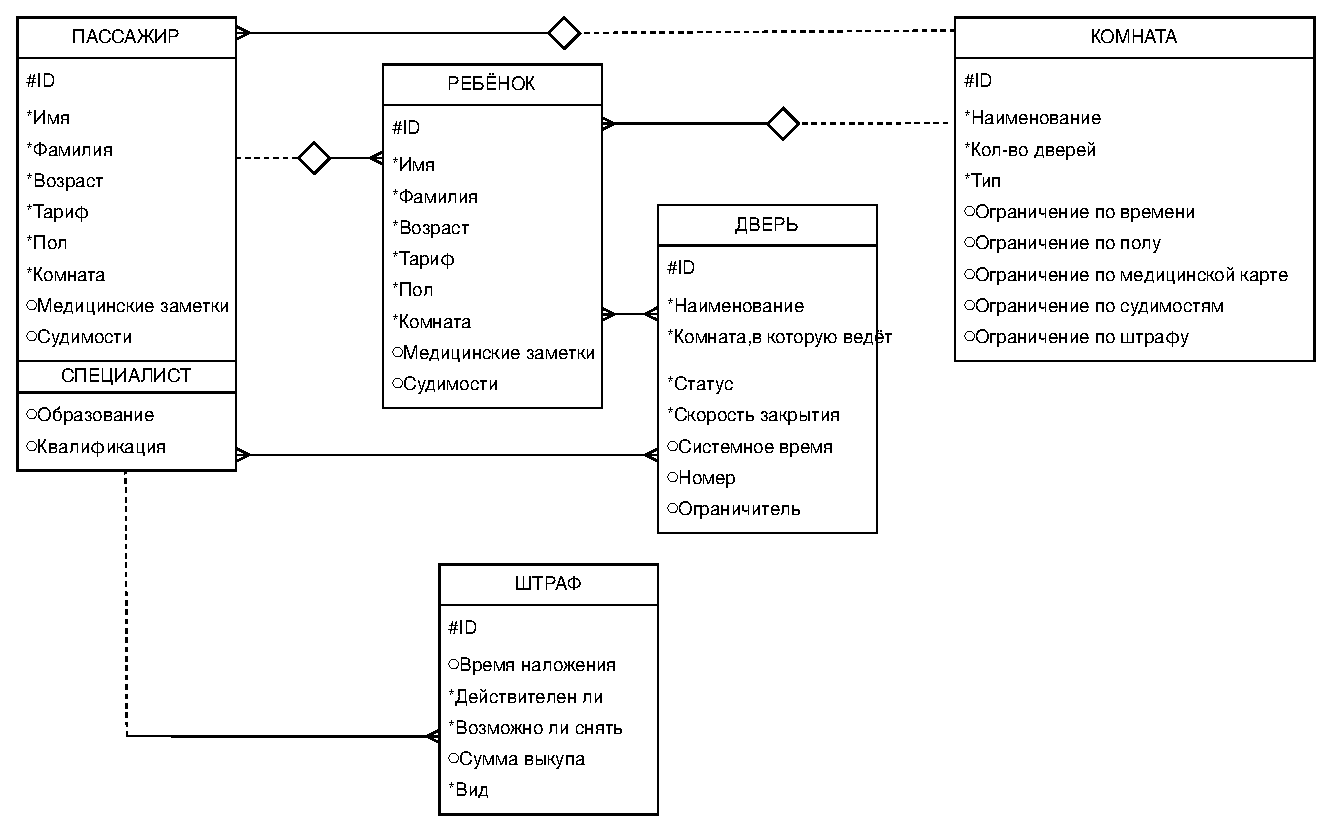
\includegraphics[width=1\linewidth]{images/ER}
	\caption{ER-диаграмма}
	\label{fig:er}
\end{figure}

\subsection{Функциональные требования к программной системе}

На основании анализа предметной области, разрабатываемая программная система «СКУД на круизном лайнере» должна включать в себя следующие ключевые функциональные возможности:
\begin{itemize}
	\item открыть/закрыть таблицу;
	\item редактировать таблицу;
	\item перейти к следующему/предыдущему элементу;
	\item добавить новый элемент -- реализация опции добавления нового элемента с последующей актуализацией этих данных в БД ;
	\item редактировать выбранный элемент -- реализация опции редактирования элемента с последующей актуализацией этих данных в БД;
	\item найти элемент по идентификатору;
	\item удалить элемент -- реализация опции редактирования элемента с последующей актуализацией этих данных в БД;
	\item запросить проверку доступа -- реализация опции запроса проверки пассажира на наличие доступа к двери.
\end{itemize}

\subsection{Варианты использования}

На рисунке  ~\ref{fig:commonscheme2} представлена диаграмма прецедентов, которая служит важным средством для систематизации функциональных требований и возможностей системы, выявляя ключевые сценарии использования. Диаграмма прецедентов изображает, как пользователи могут взаимодействовать с системой, а также помогает выявить набор основных функциональных возможностей, доступных пользователям.

При построении диаграммы вариантов использования применяется унифицированный язык визуального моделирования UML.

Каждый прецедент на диаграмме отражает отдельный путь взаимодействия в системе и представляет потенциальные действия, которые могут быть предприняты пользователями в различных ролях. Пользователем или действующим лицом является сущность, взаимодействующая с системой извне (например, человек, техническое устройство).

\begin{figure}[ht]
	\centering
	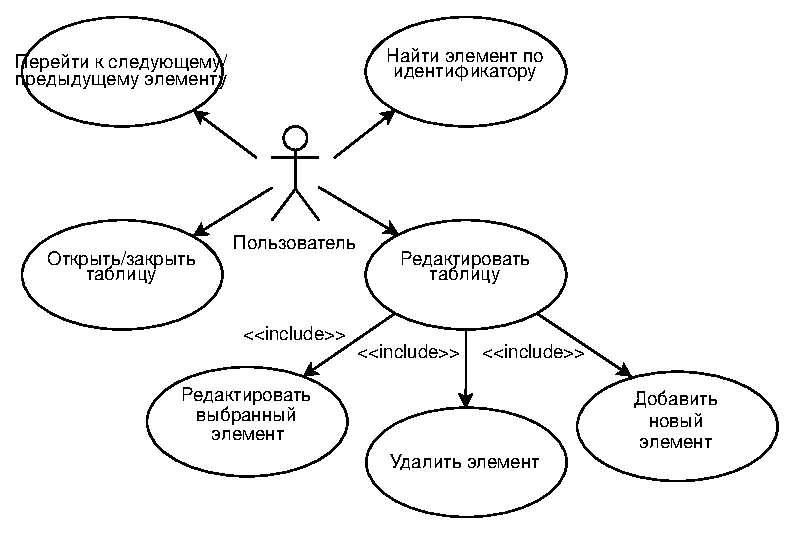
\includegraphics[width=1\linewidth]{images/CommonScheme2}
	\caption{Диаграмма прецедентов}
	\label{fig:commonscheme2}
\end{figure}

\subsubsection{Вариант использования <<Открыть/закрыть раздел данных>>}

Пользователь выбирает интересующую его раздел данных из списка предложенных и открывает окно, репрезентирующее требуемый от приложения интерфейс панели управления данными.
\subsubsection{Вариант использования <<Сменить режим работы>>}

На судне началась чрезвычайная ситуация и пользователь меняет режим работы СКУД в главном меню с помощью переключателя.

\subsubsection{Вариант использования <<Редактировать данныe>>}

Пользователь решает внести какие-либо изменения в данных. Он может сделать это, добавляя новые элементы, удаляя или редактируя существующие.

\subsubsection{Вариант использования <<Перейти к следующему/предыдущему элементу>>}

Пользователь листает элементы в таблице посредством перехода к предыдущему/следующему за текущим.

\subsubsection{Вариант использования <<Найти элемент по идентификатору>>}

Пользователь решает не листать элементы по одиночке т.к. не хочет тратить на это время. Он помнит идентификатор искомого элемента, вводит его в предназначенное текстовое поле и переходит к искомому элементу.

\subsubsection{Вариант использования <<Добавить новый элемент>>}

Пользователь заполняет поля данных будущего объекта и добавляет его в таблицу по клику.

\subsubsection{Вариант использования <<Редактировать выбранный элемент>>}

Пользователь редактирует необходимые ему поля у текущего элемента и вносит эти изменения в таблицу по клику.

\subsubsection{Вариант использования <<Удалить элемент>>}

Пользователю больше не нужен выбранный элемент и он стирает его в таблице по клику.

\subsubsection{Вариант использования <<Запросить доступ>>}

Пользователю нужно узнать, есть ли у пассажира доступ к двери. Он вводит идентификаторы пассажира и двери соответственно, затем по клику получает сообщение с информацией о наличии доступа.

\subsection {Нефункциональные требования к программной системе}
\subsubsection{Требования к надежности}
Для обеспечения надёжной работы базы данных, она должна быть приведена в нормализированный по трём формам вид:
-Первая нормальная форма (1NF)

Все атрибуты объекта ПАССАЖИР имеют только одно значение.

Все атрибуты объекта РЕБЁНОК имеют только одно значение.

Все атрибуты объекта ДВЕРЬ имеют только одно значение.

Все атрибуты объекта КОМНАТА имеют только одно значение.

Все атрибуты объекта ШТРАФ имеют только одно значение.

Все атрибуты объекта пересечения ДОСТУПЫ имеют только одно значение.

Все атрибуты объекта пересечения ДОСТУПЫ ЧС имеют только одно значение.


-Вторая нормальная форма (2NF)

Атрибуты объекта ПАССАЖИР зависят от полного UID (id пассажира).

Атрибуты объекта РЕБЁНОК зависят от полного UID (id ребёнка).

Атрибуты объекта ДВЕРЬ зависят от полного UID (id двери).

Атрибуты объекта КОМНАТА зависят от полного UID (id Комнаты).

Атрибуты объекта ШТРАФ зависят от полного UID (id штрафа).

Атрибуты объекта пересечения ДОСТУПЫ зависят от двойного UID.

Атрибуты объекта пересечения ДОСТУПЫ ЧС зависят от двойного UID.


-Третья нормальная форма (3NF)
При проверке всех объектов не было выявлено независимых от UID атрибутов или атрибутов, зависимых от других атрибутов.

На основе ER-модели данных построена реляционная модель данных, которой должна соответствовать БД. Она показанная на рисунке  ~\ref{fig:commonscheme3}

\begin{figure}[ht]
	\centering
	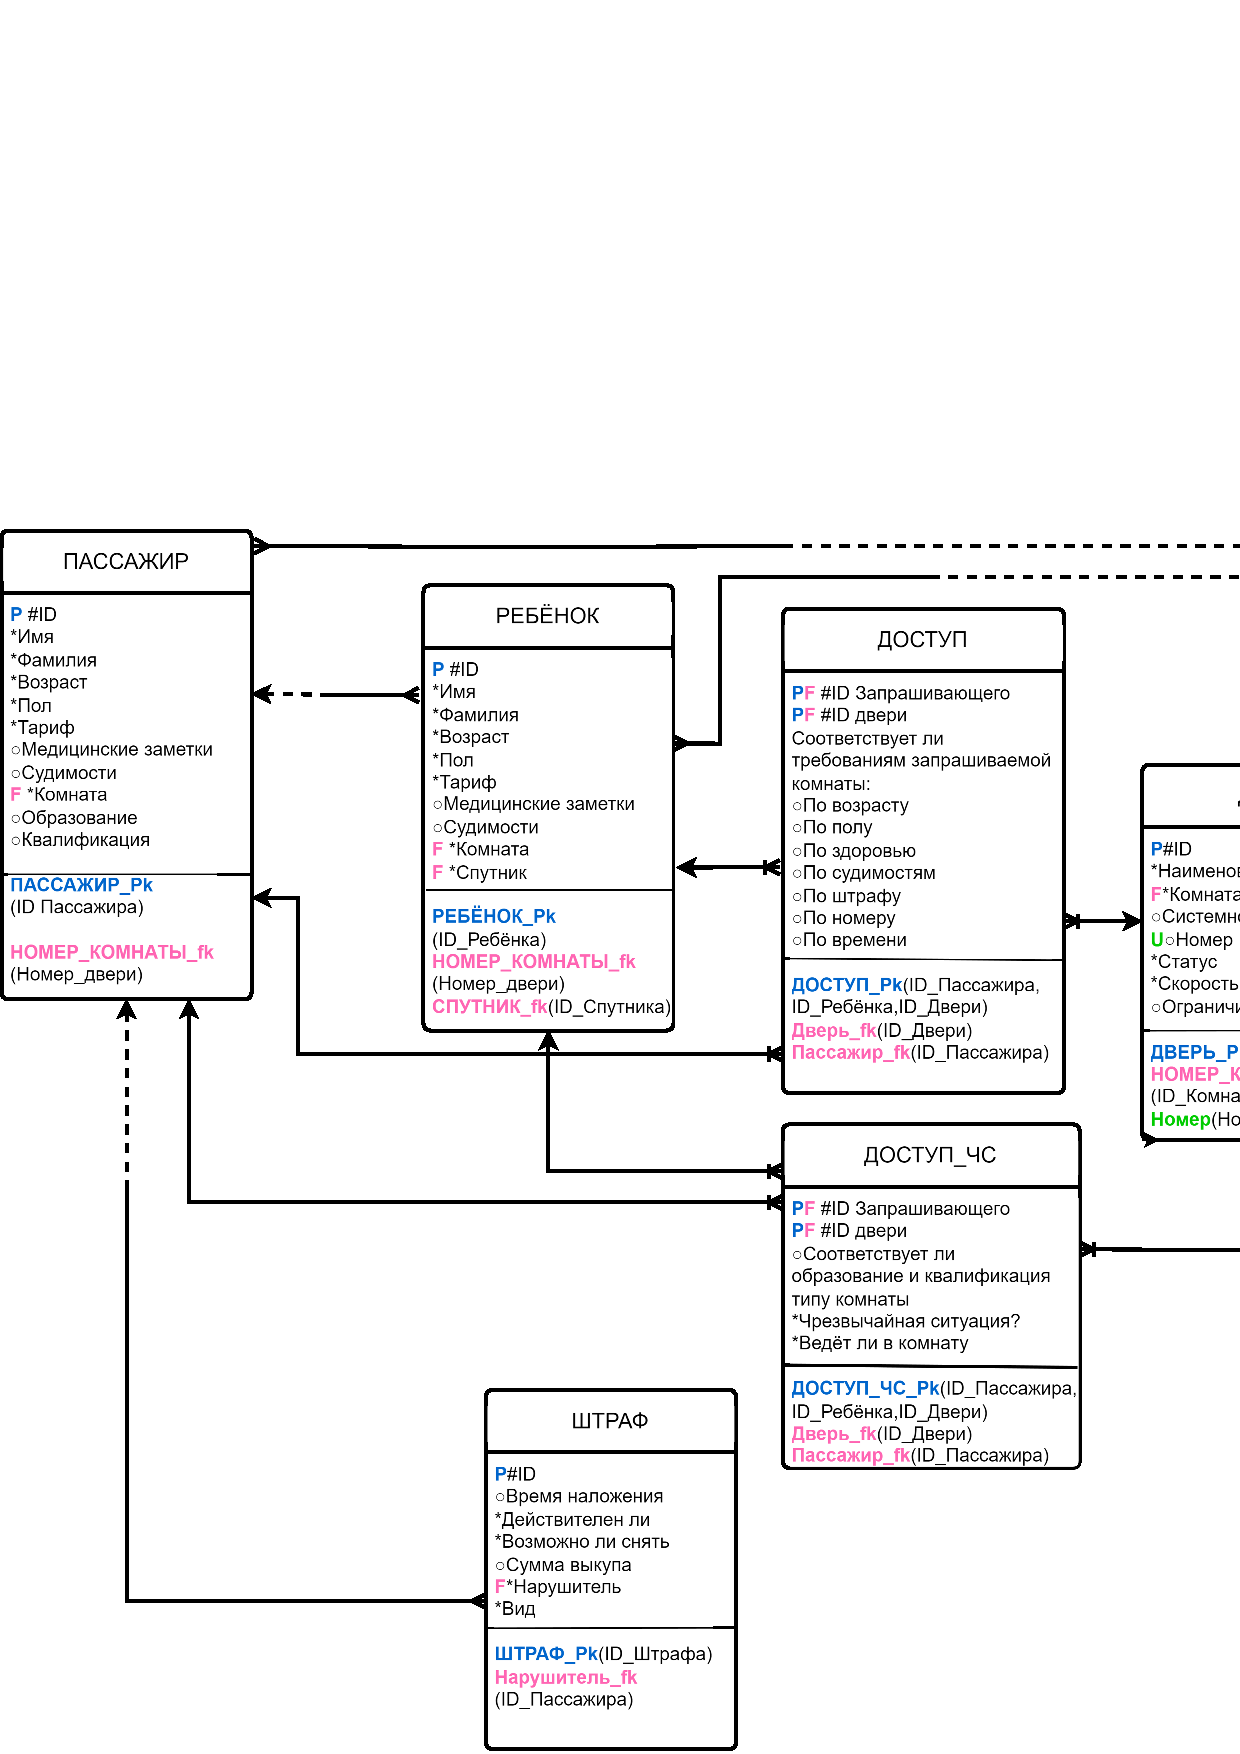
\includegraphics[width=1\linewidth]{images/CommonScheme3}
	\caption{Реляционная модель данных}
	\label{fig:commonscheme3}
\end{figure}

\subsubsection{Требования к безопасности}
1. Поддержка современных операционных систем, обеспечивающих стабильную и безопасную работу на различных платформах.

2. Регулярное обновление компонентов системы для предотвращения уязвимостей, связанных с устаревшим программным обеспечением.

\subsubsection{Требования к программному обеспечению}

Для реализации программной системы необходимо подготовить следующие компоненты:
\begin{itemize}
	\item интерпретатор языка программирования Python;
	\item СУБД SQLite.
\end{itemize}
Для работы и приложения требуется ОС Windows 7 или более поздняя версия/Ubuntu 16.0 или более поздняя версия с установленным интерпретатором языка python и установленной СУБД SQLite.

\subsubsection{Требования к аппаратному обеспечению}
Системе необходим центральный процессор с количеством ядер от 2 и выше с частотой ядра от 1.4 ГГц. Объем оперативной памяти – 4 Гб.
Свободное место на диске: 13МБ

\subsection{Требования к оформлению документации}

Требования к стадиям разработки программ и программной документации для вычислительных машин, комплексов и систем независимо от их
назначения и области применения, этапам и содержанию работ устанавливаются ГОСТ 19.102–77. Программная документация должна включать в себя:

1. Анализ предметной области;

2. Техническое задание;

3. Технический проект;

4. Рабочий проект.

